\subsection{Analysis Overview}
\label{subsec:ana_overview}
The analysis relies on Monte Carlo events that are fully simulated using the ILD detector model \url{ ILD_l5_o1_v02 } with iLCSoft version v02-00-02 and includes a complete standard model background for final states with 2,4, and 6 fermions as well standard model Higgs production.  A center of mass energy of 500 GeV and longitudinally-polarized beams in various operating scenarios are considered. The Monte Carlo events are generated for $100\%$ polarized beams, that is, either all left or right handed. Events are weighted in order to obtain realistic cases of partial polarizations for possible running scenarios which are shown in Table \ref{tab:beamscenario}.

\begin{table}
\label{tab:beamscenario}
\caption{Possible running configurations with partial beam polarizations ($P_{e^-},P_{e^+}$) and integrated luminiosity \cite{ilcop} }
\begin{tabular}{|c|c|c|c|c|}
\hline 
Pol. &(-0.8,+0.3) & (+0.8,-0.3) & (-0.8,-0.3) & (+0.8,+0.3) \\ 
\hline 
$\int$ Lum. [fb$^{-1}$] & 1600 & 1600 & 400 & 400 \\ 
\hline 
\end{tabular} 

\end{table}
 The partial polarizations $P_{e^-} \, \, P_{e^+}$  can be represented by the fraction of the beam which is either left or right handed
 \begin{equation}
 \begin{split}
f_R^{e^-} + f_L^{e^-} = 1 \, \, \, \, \, \, f_R^{e^-} = \frac{1}{2}(1 + P_{e^-}) \\
f_R^{e^+} + f_L^{e^+} = 1 \, \, \, \, \, \, f_R^{e^+} = \frac{1}{2}(1 + P_{e^+})
\end{split}
 \end{equation}
where the beam fraction $f$ is denoted with the polarization subscript and respective beam superscript. For a particular scenario like $(P_{e^-}, P_{e^+}) = (-0.8, +0.3)$ the -0.8 represents an electron beam with $90\% $ left handed electrons mixed with $10\% $ right handed electrons and a positron beam with $65\%$ right handed positrons mixed with $35\%$ left handed positrons. The weight $\omega$ for a specific event with a particular initial state helicities is given by (with example partial polarizations (-0.8,+0.3) ):
 \begin{equation}
 \begin{split} 
 \omega_{LR} = f_L^{e^-}f_R^{e^+} = 0.9 \times 0.65 = 0.585 \\
 \omega_{RL} = f_R^{e^-}f_L^{e^+} = 0.1 \times 0.35 = 0.035 \\
 \omega_{LL} = f_L^{e^-}f_L^{e^+} = 0.9 \times 0.35 = 0.315 \\
 \omega_{LR} = f_R^{e^-}f_R^{e^+} = 0.1 \times 0.65 = 0.065 
 \end{split}
 \end{equation} 

The analysis workflow for semileptonic WW has three distinct stages, the lepton identification and selection, pile-up rejection in the hadronic system, and event selection against against full standard model backgrounds. The analysis is performed with the all four running scenarios with cuts optimized for the dominant WW production mode (-0.8,+0.3). 


\subsection{Lepton Identification}
\label{subsec:Lepton_ID}
The approach towards the identification of leptons relies on treating leptons universally. The easiest lepton to identify is the muon, which produces a single track along with hits in the muon detector. The electron also produces a track in the TPC but is often accompanied by photons via bremsstrahlung radiation. The tau is the most difficult lepton to identify due to its decay into multiple charged and neutral particles. To accommodate all types lepton signatures a cone based approach is used to either capture single tracks or collimated jets with low track multiplicity. The lepton finding cone consists consists of two major structures, a search cone containing the particles that belong to the lepton candidate and an isolation cone whose purpose is to reject a lepton candidate if the search cone is not well-isolated from other particles. The acceptance criteria for cone consists of these parameters:
\begin{itemize}
\item Search cone angle $\alpha$ - The opening (half) angle of the search cone for the lepton jet [rad]
\item Isolation cone angle $\beta$ - The outer isolation cone angle w.r.t to the search cone [rad]
\item Isolation energy - The total energy allowed within the isolation cone region [GeV]
\item Invariant Mass - The upper limit on the lepton candidate mass [GeV]
\item Track multiplicity - The allowed number of tracks in a lepton candidate
\item $P_t$ seed - the minimum transverse momentum of a track that seeds a lepton candidate [GeV] 
\end{itemize}
An example of the cone and parameters are shown in Figure \ref{fig:cone}. Additional requirements are imposed on all of the reconstructed Particle Flow Objects(PFOs) in the event in order to suppress pile-up particles being included in the lepton jet.
\begin{figure}
\label{fig:cone}
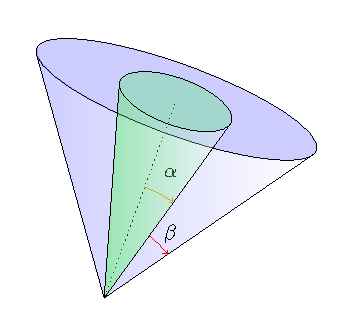
\includegraphics[width=0.3\textwidth]{cone.pdf}
\caption{Illustration of possible lepton candidate cone with search cone angle $\alpha$ and isolation cone angle $\beta$}
\end{figure}
\begin{itemize}
\item $P_t > 0.2$ GeV
\item $|cos\theta| < 0.99$
\end{itemize}
The formation of a lepton candidate follows three steps (1) candidate construction, (2) candidate merging, and (3) isolation testing.
The first step starts with a list of seed tracks sorted by energy in descending order. The track energy is calculated with respect to an assumed mass that is imposed by the Pandora PFA.  A track that qualifies as a seed track forms a new lepton candidate, any track that falls within the search cone of the lepton candidate is added to the lepton candidate. For each newly added particle the energy and momentum is updated for the lepton candidate. Tracks that have been added to a lepton candidate are removed from the track seed list. Next, the neutral particles that fall inside the search cone are added to the lepton candidate. The neutral particles also reside on a list, and are removed from the list if added to a lepton candidate, enforcing uniqueness for each lepton candidate. Lepton candidates are continually formed until the list of seed tracks exhausted. When there are no more candidates to be created, the candidates are subjected to part of the acceptance criteria: the lepton jet mass is required to be below upper mass limit (2 GeV) and the number of charged tracks within the lepton candidate is non-zero and less than or equal to 4. If a lepton jet violates any acceptance conditions it is deleted. The next step in the process is merging. If two lepton candidates fall within each others search cones, the candidates are merged. If the mass or track multiplicity conditions are violated, both lepton candidates are deleted.  All  candidates that survive merging are subjected to the isolation testing. For each candidate, the sum of energy of all the particles that fall inside the isolation cone is computed. If the total energy inside the isolation cone is greater than the maximum allowed energy inside the isolation cone the lepton candidate is deleted.\\
\quad \quad \\
The universal lepton treatment is not conducive to a 1-size fits all approach to lepton ID due to the abundance of different lepton signatures. To accomodate for variations between leptons signatures, the acceptance criteria for leptons is optimized according to lepton flavor and $\tau$ decay topology. The categories created are:
\begin{itemize}
\item Prompt $\mu$
\item Prompt $e$
\item $\tau \rightarrow \mu \bar{\nu_{\mu}} \nu_{\tau} $
\item $\tau \rightarrow e \bar{\nu_{e}} \nu_{\tau} $
\item $\tau \rightarrow$ hadrons (1-prong)
\item $\tau \rightarrow$ hadrons (3-prong)
\end{itemize} 
The Prompt categories refer to events which the leptonic W decays directly to either a muon or electron and associated neutrino. The tau categories address the various dominant decay topologies of the tau lepton. For each category, the optimal lepton acceptance criteria is calculated with respect to the events that match the desired topology. The optimal acceptance criteria is the set of parameters that maximally identify lepton candidates that originate from true leptons and minimize the fake lepton candidates that originate from hadronic jets. To find this set of parameters, a scan over a 3D space is performed using the search cone-$\alpha$, isolation cone-$\beta$, and isolation energy-$E_{iso}$. The invariant mass is held at a fixed 2 GeV for simplicity. The ranges and step sizes through this space are:
 \begin{itemize}
 \item $\alpha \in [0,0.15]$ rad with 0.01 rad steps
 \item $\beta \in [0,0.15]$ rad with 0.01 rad steps
 \item $E_{iso} \in [0,5.5]$ GeV with 0.5 GeV steps
 \end{itemize}
Two uncorrelated push-pull parameters are defined to find the optimal working point in the lepton finding space. The first is related to correctly identifying jets originating from true leptons. This is denoted as the efficiency of reconstructing a true lepton $\epsilon_T$. The second optimization parameter is denoted as $P_F$, the probability of a fake lepton jet arising from a single hadronic jet.  
\begin{equation}
\label{eq:et}
\epsilon_T = N_{match}/N_{Stotal}
\end{equation}
\begin{equation}
\begin{split}
\label{eq:pf}
P_F = 1-(1-\epsilon_F)^{\frac{1}{4}} \\
\epsilon_F = N_{fake}/N_{Btotal}
\end{split}
\end{equation}
The true lepton reconstruction efficiency is maximized with the signal sample $WW\rightarrow q\bar{q}\ell\nu$. The denominator represents the total, category specific, number of events which contain three generator visible fermions. The true $q\bar{q}\ell$ fermions are required to fall within the acceptance range $|cos\theta| < 0.99$. $N_{match}$ is the number of signal sample events in which a lepton candidate is reconstructed and can be matched to the true lepton, such that the opening angle between the reconstructed lepton and the true lepton are less than 0.1 radians. The distribution of opening angles is shown if Figure X. In the case that a reconstructed lepton is being matched to a true tau, the matching angle formed between the reconstructed lepton and the vector sum of the visible generator components of the tau decay. The visible components of the tau decay consist of the direct decay products whereas photons from final state radiation are excluded. The fake lepton probability $P_f$ is minimized using the background sample $WW\rightarrow q\bar{q}q\bar{q}$ and is a function of the fake lepton reconstruction efficiency $\epsilon_F$. The denominator for fake is also subjected to the same acceptance range $|cos\theta| < 0.99$ for all four fermions. The numerator is the total number of events  that contain at least one reconstructed fake lepton. The fake efficiency can be interpreted as the binomial probability of $r$-successes(lepton reconstructions) in 4 trials(hadronic jets). The probability of a single success in a single trial, $P_F$, can be directly derived from the Binomial p.d.f using the fake efficiency $\epsilon_F$. The optimal parameters $\alpha$, $\beta$, $E_{iso}$ for each lepton category are extracted from max$[(1-P_F)\epsilon_T]$. The results for each category are shown in Table X. 

Since there is only one expected lepton jet in the signal sample, a single lepton jet is selected as the candidate for the event. If there are multiple lepton jets reconstructed in a single event the lepton jet with the highest energy is selected as the single candidate for the event. The Energy distribution of true and fake leptons is shown in Figure X. If the two highest energy lepton jets are of equal energy then the candidate selected will be the jet with the highest energy original seed track, based on the original seed track sorting.  Any additional lepton jets that are not selected are treated as part of the hadronic system.


\subsection{Pileup mitigation}
\label{subsec:Pileup_mitigation}
Following the lepton selection the remaining particles in the system are expected to form the hadronically decaying W boson. However, the sum of the four momenta of the paricles  produces a distrbution that is often greater than the true hadonic mass. Figure X shows the systematic mismeasurement of the hadronic W mass. Small variations between the true W mass and measured W mass naturally arise due to the mismeasurment of particles -- specically neutral hadrons. If the diffence between the measured and true W mass is signifcantly negative it means that hadronic particles have been lost due to acceptance.  Events in which the difference between the measured and true W mass is significantly positive indicates that the hadronic system contains particles that are not associated with the WW process i.e. pileup.   To combat the measuerment excess due to pileup jet clustering algorithms via FastJet\cite{fastjet} are used.  The standard approach for pileup mitigation is to use the kT algorithm\cite{kt} and tune the R parameter such that the pileup particles are associated with beam jets while the desired particles are associated to non beam jets. With successful kT clustering the beam jets can be thrown away without damaging the reconstruction of the desired event. However, this approach only works well in events that are centrally produced.  The leading cross-section of WW in the $e^{-}_L e^{+}_R$ polarization yields an kinematic topology where the down like quark tends to be boosted forward causing overlap between the jet particles and pile-up particles. In this topology employing the kT algorithm leads to rejecting desired particles and severe undermeasuremnt of the the W mass. The solution to proper pileup mitigation is through jet fragmentation.   Using the standard JADE algorithm which has no beam jet association and uses the mass based cutoff parameter $y_{cut} > y_{ij}$ where $y_{ij} = M_{ij}^2 / Q^2$ with $M_{ij}$ being the invariant mass of the pair of objects being combined and $Q^2$ being the visible energy in the $e^{+}e^{-}$ annihilation \cite{ycut}. By tuning the $y_{cut}$ parameter the mass of individually reconstructed jets can be controlled. For large ycut values O(1e-3) a single massive jet is reconstructed and in the limit that ycut becomes infinitely small the number of jets reconstructed is the number of reconstructed particles.  The ycut value  chosen is the value that forms mini-jets that safely couple together hard and soft emissions from  the original parton while segregating pile into its own mini-jets. The mini-jets are then subjected to kinematic cuts that are chosen to maximize the pileup rejection and minimize the rejection of true W daughter particles. The optimal ycut and mini-jet kinematic cut combination are selected over the range
\begin{itemize}
\item $y_{cut} \in [1\times 10^{-3}, 0.5\times 10^{-3}, \ldots , 4.5\times 10^{-6}, 5\times 10^{-6}$
\item mini-jet $pT < x $ where $ x \in [0,5]$ in bins of 0.5 GeV
\item mini-jet $|cos\theta| < y $ where $y \in [0.9, 1]$ in 0.01 bins
\end{itemize}
The optimization parameters used to select best combination are two statisical estimators from the distribution of $M_{qq}^{meas} - M_{qq}^{true}$. This binned mass difference distribution is created from the subset of mini-jets that arise from clustering with a given $y_{cut}$ and and also pass some jet veto cut $x$ and $y$. The estimators are the Full Width Half Maximum(FWHM) and the number of entries in the Mode.  
Using estimators calculated from a binned histogram creates unwanted sensitivity to bin size. To workaround this feature various tricks are employed. First the mode is defined as the center of the bin with the most entries the mode entries is the number of entries in the mode bin plus the number of entries in the mode bins nearest neighbors. For the FWHM, the mass distribution is assumed to be monotonically decreasing around the half maxmimum. 


\subsection{EventSelection}
\label{subsec:EventSelection}